\chapter{Framework Design}

Building DSLs is useful in achieving many software qualities. In case of library building, some of the benefits include:  
\begin{itemize}
    \item More readable definitions for mathematicians 
    \item Better customizable definitions for user of mechanized systems 
    \item Less labor from the side of library developers 
    \item Better maintainability of library 
\end{itemize}

The interpreter of a DSL transforms declarative expressions into definitions acceptable by a host language. We suggest an interpreter that consists of three phases as shown in Figure~\ref{fig:staged-interpreter}. 
\begin{figure}
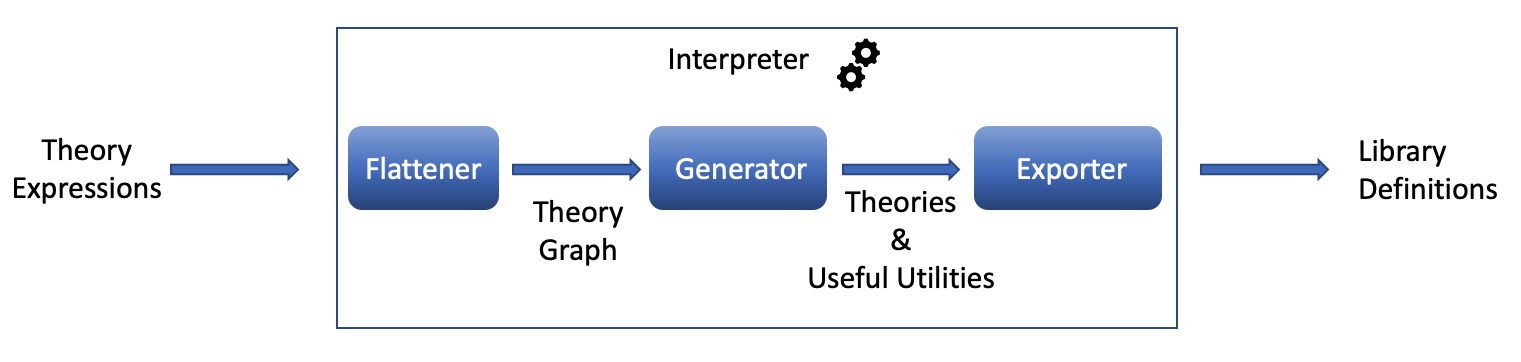
\includegraphics[scale=0.5,width=\linewidth]{figures/interpreter_detailed}
\caption{A $3$-staged interpreter for generating libraries}
\label{fig:staged-interpreter}
\end{figure}

\paragraph{Flattener.} The first stage of the interpreter take in theory expressions and computes a flat version of the theory being described. The theory expressions need to be designed well enough to describe the structure of mathematics, i.e. build a theory graph paying special attention to morphisms that describes how theories relate to each other. Describing this structure is useful in transporting results, but mathematical results are not always shaped in terms of the hierarchy. A \lstmath{Group} can be described as a \lstmath{Monoid} with inverse or as a structure with binary and unary operatoins that have some properties. Our library need to support both definitions, by enabling the users to work with flat version of the library. Some operations on theories make this hard to achieve, like dropping and freeness combinators by CASL\ednote{look for a source explaining why they are problematic}. 
\ednote{add a figure?}

\paragraph{Generator.} When we have a flat theory presentation describing an algebraic structure, we check if this theory falls under the abstraction provided by universal algebra. The algebraic hierarchy until at least \lstmath{Ring}\ednote{or maybe more?} does. If so, then we are able to generate the constructions that universal algebra describes based on that abstraction. 

\paragraph{Exporter.} Variabilities in the design decisions between different systems affects how theory presentations look like. At the end of the day, those variabilities are translated into syntactic differences. By abstracting over them, we are able to remove or add them upon the developer's will. It is the job of the exporter to do that, providing a version of the theory that fits best the users' purposes. 



